\setchapterpreamble[u]{\margintoc}
\chapter{Annual analysis: Andasol-II \gls{cspLabel} plant}%\gls{cspLabel} and inland-MED}
\labch{cc:simulation}

\tldrbox{ This chapter presents an analysis of the annual performance of
    different cooling alternatives applied to a commercial 50~MW$_e$
    \gls{cspLabel} plant, Andasol-II, located in southern Spain. Three cooling
    systems are compared: the actual cooling system of the plant, a
    \gls{wctLabel}, the proposed combined cooling system (\gls{ccLabel}) with
    two different capacities for the dry cooler, 75\% and 100\% of the nominal
    thermal load of the \gls{wctLabel} system. For each alternative the
    operation is optimized in a water-scarce scenario using the proposed
    multi-stage optimization framework, adapted to the particular case study. 

    Results show that integrating the \gls{ccLabel} can reduce specific cooling
    costs by up to 80\% and annual water consumption by about 48\%, with 38\%
    savings during the driest months. These benefits arise from reduced dependence
    on costly alternative water sources. The \gls{ccLabel} alternatives also
    provide more stable, cost-effective operation across the year compared to the
    \gls{wctLabel}, which is highly sensitive to water scarcity. Overall, the study
    demonstrates that optimized combined cooling can significantly enhance both
    economic and water-use efficiency in \gls{cspLabel} plants.
}

\section*{Introduction}
\addcontentsline{margintoc}{section}{Introduction}

\begin{marginfigure}[*-6] % -5.5cm
    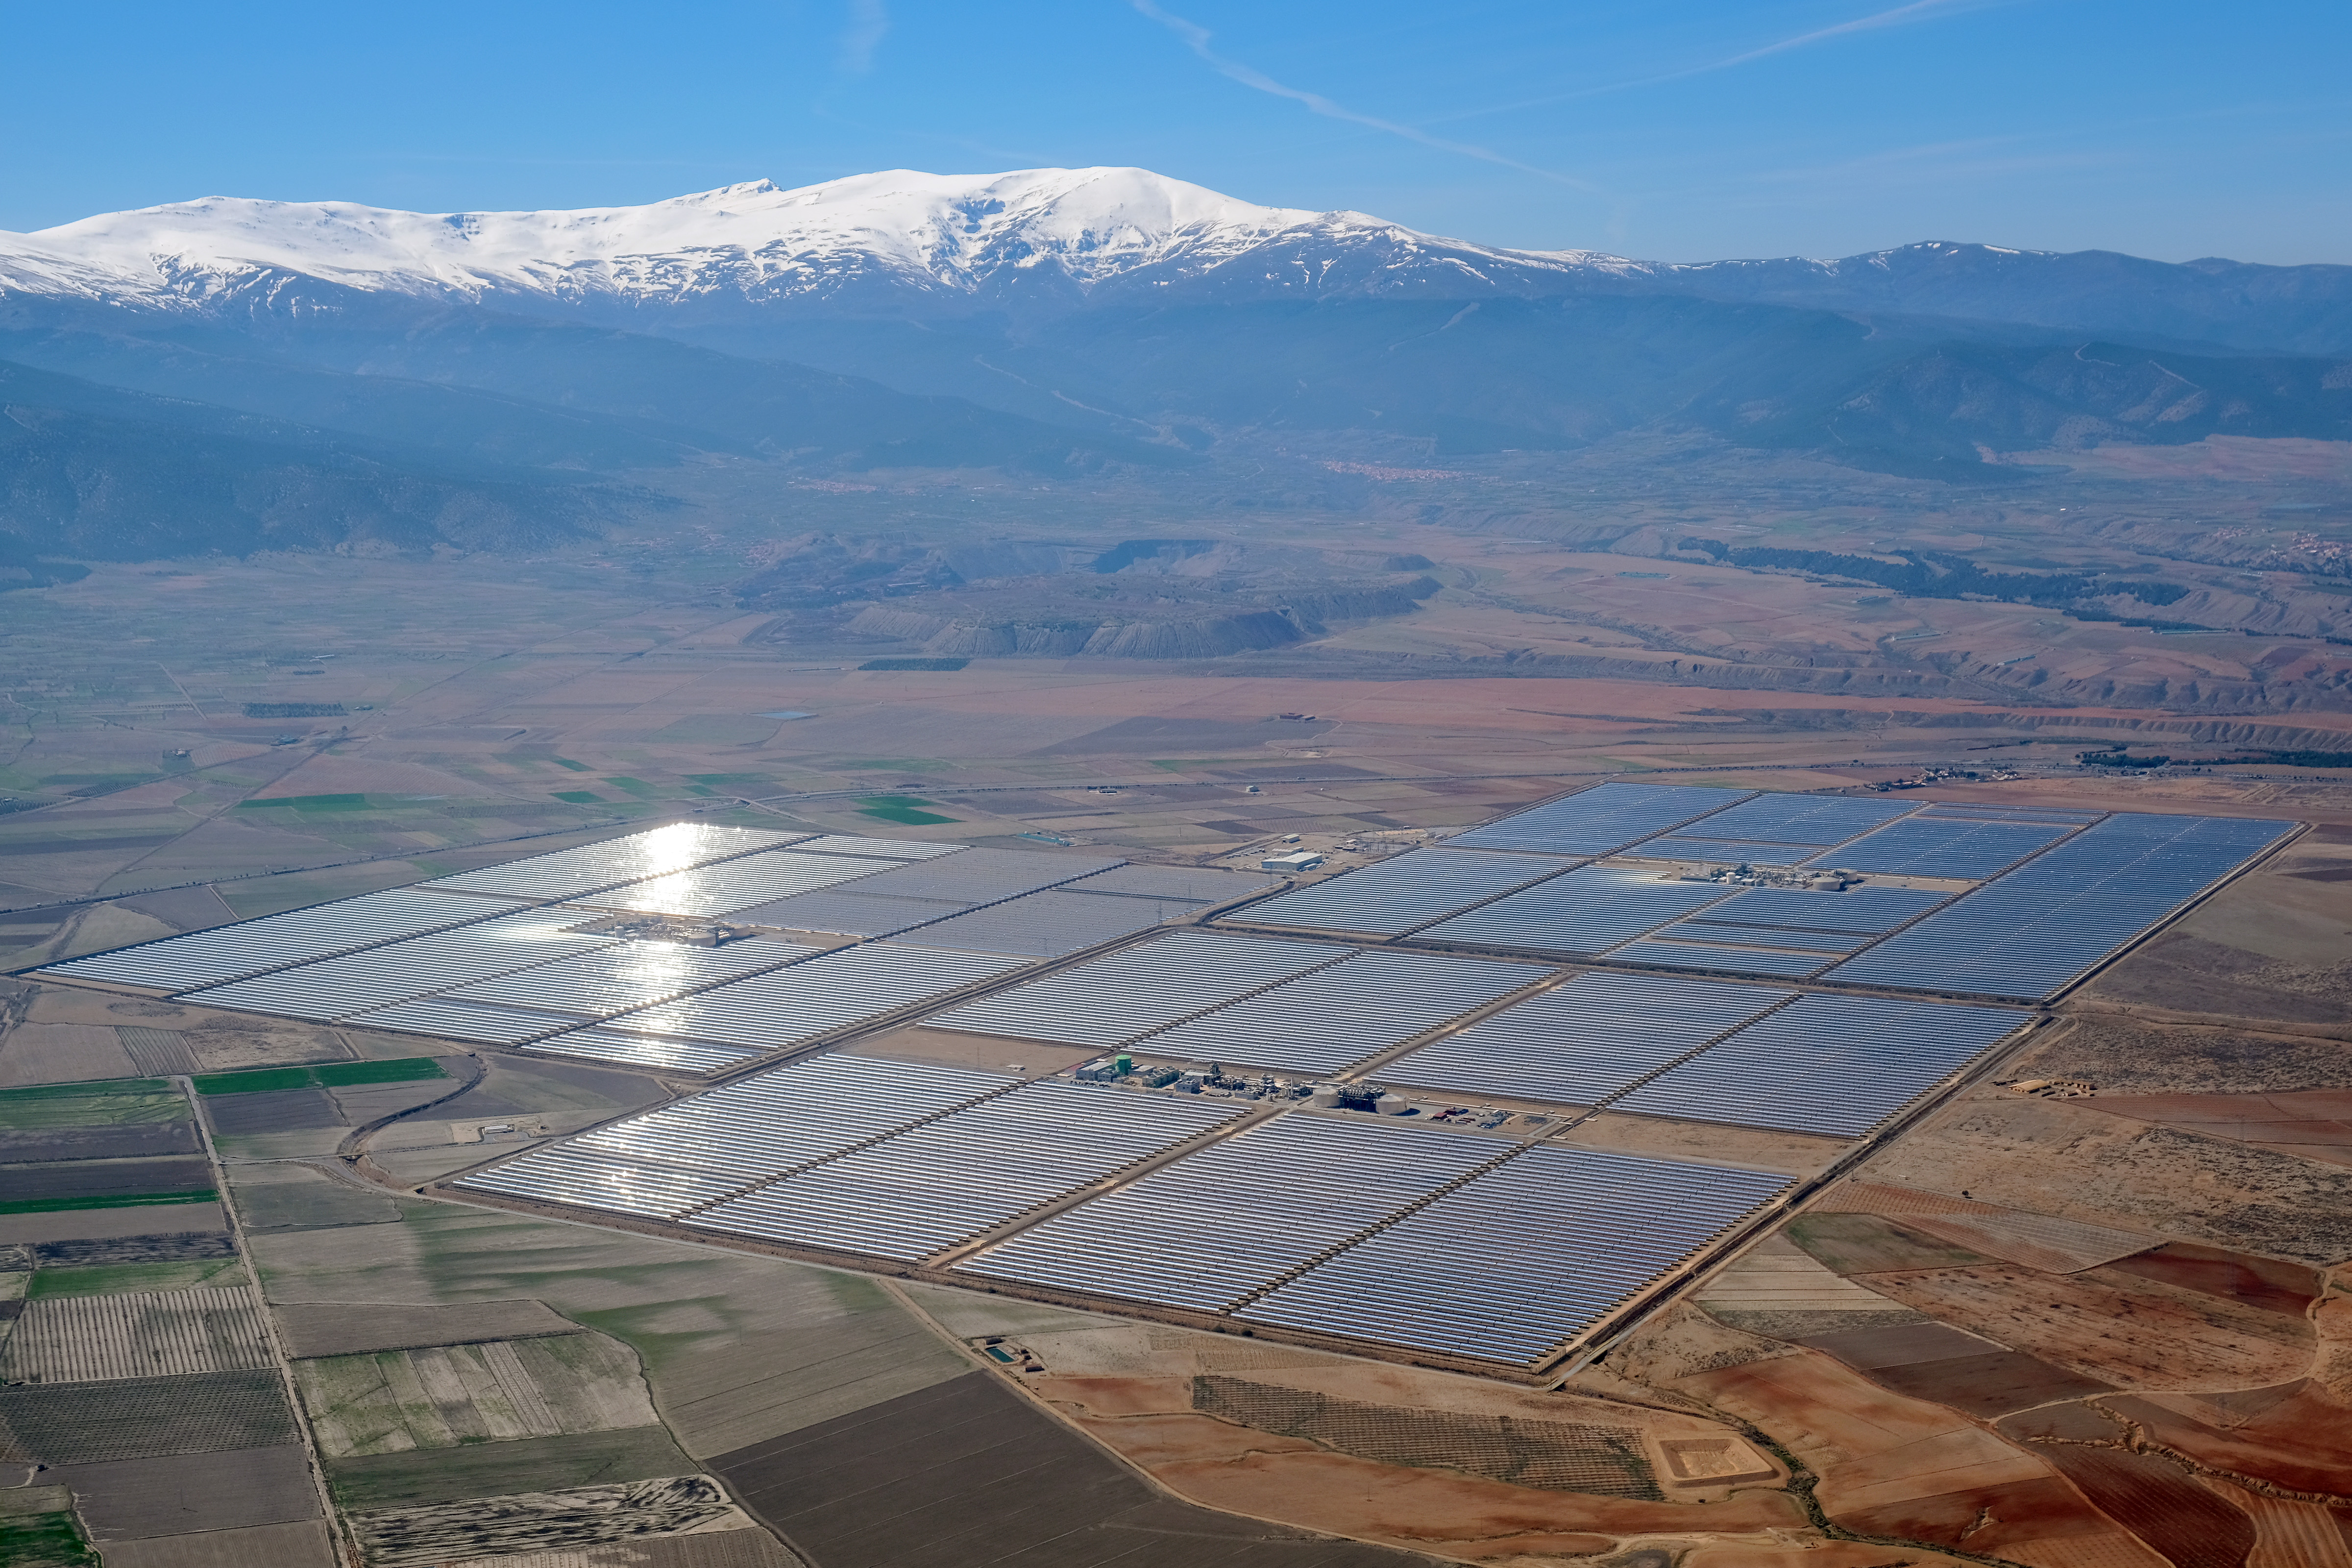
\includegraphics[]{andasol.jpg}
    \caption[Andasol I, II and III]{Andasol I, II and III aerial view.
    Andasol-II is the one at .\\ 
	{\tiny Source: \url{https://en.wikipedia.org/wiki/File:Andasol_5.jpg}}}
    \labfig{cc:simulation:andasol}
\end{marginfigure}

% Introducción
A modeling framework has been developed to simulate and optimize the operation
of various cooling systems, with a particular focus on the proposed combined
cooling system. This methodology has been validated using data from a pilot
plant. In this chapter, the objective is to apply the framework to a specific
case study: a commercial 50~MW$_e$ \fullgls{cspLabel} plant.

As previously mentioned, \gls{cspLabel} plants are among the most water-intensive power
generation technologies, a concern that is especially relevant in the arid
regions where they are typically located. To assess the performance ---water use
and operational costs--- of different cooling systems, the proposed methodology is
applied to a real-world case study through an annual simulation. The case study
examined is the Andasol-II \gls{cspLabel} plant.

% Descripción ANDASOL
In the south-east of Spain, near Guadix and next to the Sierra Nevada mountain
range (see \reffig{cc:simulation:andasol}), thanks to the region high altitude
(1100~m) and the semi-arid climate, the site has exceptionally high annual
direct insolation (2260~W/m$^2$) and thus is ideal for solar projects. This is
why the first parabolic trough power plant in Europe, Andasol-I, was built there
in 2008. One year later Andasol-II followed, located in the immediate
neighbourhood and with almost identical construction. It has a rated output of
50~MW with 7.5~hours\sidenote[][*-14]{This means that if fully charged, it can
produce the nominal rated power of the turbine for that duration} of thermal
storage, providing electricity for up to 200,000 people. According to the
developer, Andasol-II vaporizes 870 000~m$^3$/year, or in specific units
\textbf{5~l/kWh}. More specifications are available in
\reftab{cc:simulation:andasol}.

\begin{margintable}[*-15]
    \caption{Andasol-II plant main characteristics}
    \labtab{cc:simulation:andasol}
    \resizebox{\linewidth}{!}{
    \begin{tabular}{|l|l|}
        % \toprule
        % \textbf{Parameter} & \textbf{Value} \\
        % \midrule
        Technology & Parabolic Trough \\
        Solar Resource & 2260 W/m$^2$ \\
        Nominal Capacity & 50 MW \\
        Status & Operational \\
        Start Year & 2009 \\
        Expected Generation & 158 GWh/year \\
        Total Land Area & 2 km$^2$ \\
        LCOE (2020) & 0.27 €/kWh \\
        TF Inlet Temperature & 293$^\circ$C \\
        TF Outlet Temperature & 393$^\circ$C \\
        Power Cycle & Steam Rankine \\
        Turbine Efficiency & 38.1\% \\
        Cooling Type & Wet \\
        Storage Type & Molten salts \\
        Storage Capacity & 7.5 Hours – 1 GWh \\
        % \bottomrule
        % \multicolumn{2}{l}{} \\
    \end{tabular}
    \vspace{0.5em}
    }
    \scriptsize \textcolor{black!50!gray}{Source: Institute for Advanced Sustainability Studies (IASS) and others, 2022; data by Lilliestam@IASS, Thonig@IASS, Zang@CAS, Gilmanova@CAS and others. Licensed under a \href{https://creativecommons.org/licenses/by/4.0/}{Creative Commons Attribution 4.0 International License}.}
\end{margintable}

% Estructura del capítulo


%===================================
%===================================
\section{Environment definition}
\labsec{cc:simulation:environment}


%================================
\subsection{Water context}
\labsec{cc:simulation:environment:water}

Obtaining accurate water availability data is challenging. Unlike resources
such as electricity ---where demand, supply, and prices are readily
available--- water availability data is often lacking. Water prices are not
standardized; they vary from region to region, and even within the same region,
depending on the source and the specific agreements in place.

For the simulation scenario, two sources of water are considered\sidenote{See
\nrefsec{cc:optimization:environment}}. The first source is rainwater
collected in a reservoir, which is assumed to be available at a constant price. To
create a representative dataset, water availability is modeled as a function of
precipitation data, which can be obtained from hourly \gls{tpyLabel}
data~\sidecite{meteotestag_meteonorm_}. A linear model is fitted to relate
maximum precipitation to maximum available water, and when there is no
precipitation, water availability is set to zero. The data is then resampled
every 15 days, and the daily volume of available water is calculated by dividing
the resampled fortnightly volume by 15. This approach accounts for the presence
of water reservoirs and some degree of management capacity.

The alternative regenerated water source\sidenote{This is not an exogenous
idea; the Villena \gls{cspLabel} plant, for example, uses wastewater from a nearby prison
to partially meet its water needs} is not limited in volume.

%================================
\subsection{Thermal load}
\labsec{cc:simulation:environment:load}

Traditionally, thermal power plants were designed and operated to generate
electricity only when solar energy was available. This approach remained common
until the rapid rise in competitiveness of \gls{pvLabel} plants, which offer
significantly lower generation costs. In response, concentrated solar power
plants began integrating thermal energy storage systems to enable dispatchable
power generation. Today, 21 out of 51 \gls{cspLabel} plants in Spain—approximately
42\%—have thermal storage capacities exceeding two
hours~\sidecite{thonig_cspguru_2023,lilliestam_midterm_2021,bonilla_csp_2024}.
This enables them to produce electricity even when solar input is unavailable.

However, many of these plants still follow traditional operating patterns,
generating most of their electricity during peak solar hours\sidenote{The
storage is primarily used to extend generation past sunset.}. This strategy is
increasingly seen as suboptimal and is likely to be phased out as the electric
grid becomes saturated with \gls{pvLabel} generation\sidenote{This trend is
already observable in Spain during the summer months; see
\reffig{cc:simulation:mix}}.

% Poner figura de presentación con datos de REE
% \begin{figure}
%     \includegraphics[width=\textwidth]{spanish-electric-mix-20240712.png}
%     \caption{Spanish electricity mix on July 12, 2024. The peak in
%     photovoltaic generation is clearly visible at midday, while thermosolar
%     generation is more evenly distributed throughout the day. Peak production
%     is majorly from \gls{cspLabel} plants with no storage.\\
%     {\scriptsize \textcolor{black!50!gray}{Data source: Figure elaborated using data
%     extracted from \url{https://www.ree.es/es/datos}}}}
%     \labfig{cc:simulation:mix}
% \end{figure}


In this work, a different operational strategy is adopted: the plant is
configured to generate electricity during off-peak solar hours, typically in
the evening when electricity demand is at its highest. This is achieved by
shifting the plant's production to align with these peak demand periods.

A model of the Andasol-II plant, developed by Bartolomé~\etal~\sidecite{ortegadelgado_theoretical_2016}, was
configured to follow this production strategy and simulated over an entire
year. The resulting thermal load profile represents the demand to be met by the
cooling system. The simulation used the same weather dataset as that employed
for modeling the cooling system.


%================================
\subsection{Prices context}
\labsec{cc:simulation:environment:costs}

% \qrcode[hyperlink,height=0.5in]{https://api.esios.ree.es}\\ \href{https://api.esios.ree.es}{https://api.esios.ree.es}

\textbf{Electricity}. The spanish grid operator \gls{reeLabel} provides an
API~\sidecite{REE_website} to access the electricity market prices. A python
script was developed to systematically download monthly data\sidenote{Longer
periods would result in silent errors in the API} for each month in the desired
year. The data is fetched in hourly intervals and saved in JSON format, then
every file is read and joined into a single dataset resulting in prices for the
whole year. 

\textbf{Water}. Rainwater has a constant lower price of
$P_{w,s1}=0.03$~\euro/m$^3$. This price was obtained considering that the
plan has access to the same water than the irrigation community of the area. The
alternative source, \ie regenerated water, is considerably more expensive, and
its price is linked to the electricity price, specifically by a factor of 80:
$P_{w,s2}=80\times P_{e} = 8\pm 5$~\euro/m$^3$.%\sidenote{This value includes
% a scaling factor}.

\begin{kaobox}[title=Simulation data and parameters information] 
    \begin{itemize}
        \item \textbf{Weather data}. Hourly weather data from \gls{tpyLabel} of
        Guadix (Spain) for the year. Data from~\cite{meteotestag_meteonorm_}.
        \item \textbf{Thermal load}. Hourly thermal load data from the power block
        of Andasol-II \gls{cspLabel} plant from a simulation model~\cite{ortegadelgado_theoretical_2016}.
        \item \textbf{Electricity price}. Spanish electricity pool market for
        2022~\cite{REE_website}.
        \item \textbf{Maximum available water}. 2~m$^3$/day, modeled as a
        function of precipitation data.
        \item \textbf{Alternative water source factor}. $P_{w,s2}=80\times P_{e}$ 
    \end{itemize}
    
    % \raggedright
    % \begin{tabular}{m{0.3\textwidth} c} 
    %     The full environment dataset is available at  &
    %     \qrcode[hyperlink,height=0.5in]{\solhycoolRepositoryBaseUrl/data/datasets/environment_data_andasol_20220101_20241231.csv}
    % \end{tabular}
\end{kaobox}

\section{Cooling alternatives comparison}[Alternatives comparison]
\labsec{cc:simulation:alternatives-comparison}


The results presented in \reffig{cc:simulation:year-specific-analysis} highlight the
potential benefits of integrating the proposed combined cooler into the
Andasol-II power plant, particularly under water-scarcity conditions. The
comparison between the \gls{wctLabel} baseline and the \gls{ccLabel}
alternatives shows a remarkable reduction in the specific cooling cost: the
\gls{ccLabel} achieves reductions of around 80\% compared to the \gls{wctLabel}
reference case.  

This cost improvement is mainly explained by the reduced reliance on the
alternative water source, which dominates the cooling cost in the \gls{wctLabel}
configuration. By introducing the combined cooler, annual water consumption is
reduced by 48\% on average, and by 38\% during the most critical driest and
hottest months (see \reffig{cc:simulation:year-comparison}). This demonstrates
the ability of the \gls{ccLabel} to alleviate water stress without compromising
cooling performance.  

\begin{marginfigure}[*-12]
    \includegraphics[]{cc_year_analysis_composite_cooling_costs.png}
    \savebox\captionqr{\qrcode[hyperlink,height=0.4in]{\repositoryBaseUrl/figures/cc_year_analysis_composite_cooling_costs.html}}
    \caption[Specific cooling costs comparison]{Composite specific cooling costs comparison.\\[1ex]\usebox\captionqr}
    \labfig{cc:simulation:year-specific-analysis}
\end{marginfigure}

The figure also emphasizes the importance of comparing cooling system
alternatives under representative annual operating conditions and not just
analyzing annual averages. The \gls{wctLabel} option exhibits much higher
sensitivity to water availability, with sustained high associated costs through
most of the year and negligible on periods of water abundance. The \gls{ccLabel}
options (both at 75\% and 100\% DC capacity) provide stable and cost-effective
operation across most of the year, only penalized in the most challenging (June
- September) period and to a much lower degree compared to the \gls{wctLabel}.  


These findings confirm the need for optimization strategies in hybrid or
combined cooling systems, where the optimized operation schedule can further
improve both cost efficiency and water savings. The proposed multi-stage
optimization framework can be adapted to other plant configurations and extended
to different boundary conditions and resource availability scenarios, enabling
informed decision-making for sustainable power plant operation.  

One caveat that no optimization strategy can fully overcome is the natural
mismatch between water availability and cooling needs: in most locations,
ambient temperatures are lowest (favoring dry cooling) when water is most
available, whereas in the hot-dry summer season, water scarcity coincides with
the highest cooling demand (see \reffig{cc:simulation:year-comparison}).
Nevertheless, as shown, there remains significant margin for improved water
management through system optimization with integrated dry and wet cooling.
Moreover, \gls{cspLabel} systems could consider not operating during the hottest
hours of summer days—when water is scarce and other renewable generation is
plentiful—and instead prioritize production during off-peak hours, when cooling
is more efficient and renewable supply is lower.  

Finally, it is clear from the results that water can be the dominant cost
driver, and thus the most limiting resource depending on the location and chosen
cooling solution. For the analyzed case study this is true even when assuming a
conservative alternative water source cost of $\approx$0.08~\euro/l. Much higher
values could be expected: in discussions with the Villena \gls{cspLabel} plant
O\&M team, they indicated figures above 1~\euro/l for such alternative
sources can be expected, which would further strengthen the case for
water-efficient cooling strategies.

\begin{figure*}[h!]
    \includegraphics[width=1\linewidth]{cc-simulation-annual-comparison.png}
    \savebox\captionqr{\qrcode[hyperlink,height=0.5in]{\repositoryBaseUrl/figures/cc-simulation-annual-comparison.html}}
    \caption[Annual simulation results for the different studied alternatives optimized]{Annual simulation results for the different studied alternatives optimized
    with the proposed horizon optimization. Results are resampled every 15 days using their
    mean values.\\ \usebox\captionqr}
    \labfig{cc:simulation:year-comparison}
\end{figure*}
